\documentclass[12pt]{article}


\usepackage{amssymb}
\usepackage{amsmath}
\usepackage{fullpage}
\usepackage{epsfig}
\usepackage{epstopdf}
\everymath{\displaystyle}
\usepackage{enumerate}

\newif\ifans

\ansfalse

\begin{document}

\begin{center}
\underline{\LARGE{Chapter 3.4: Trigonometric Identities}}
\end{center}

\subsection*{Expected Skills:}

\begin{itemize}

\item Be able to derive Pythagorean Identities relating tangent/secant or cotangent/cosecant from $\sin^2\theta+\cos^2\theta=1$.

\item  Given the identities $\sin(\alpha+\beta)$ and $\cos(\alpha+\beta)$ be able to derive the double angle formulas and power reducing formulas (as described in the course notes).

\item Be able to use the Law of Cosines to relate the sides lengths of a triangle with one of the angles.

\end{itemize}

\subsection*{Practice Problems: }

\begin{enumerate}

\item Find the exact values of each of the following:

\begin{enumerate}

\item $\sin15^\circ$ and $\cos15^\circ$.

\ifans\fbox{$\sin15^\circ=\frac{\sqrt{6}-\sqrt{2}}{4}$ and $\cos15^\circ=\frac{\sqrt{6}+\sqrt{2}}{4}$} \fi

\item $\sin165^\circ$ and $\cos165^\circ$.

\ifans\fbox{$\sin165^\circ=\frac{\sqrt{6}-\sqrt{2}}{4}$ and $\cos165^\circ=-\,\frac{\sqrt{6}+\sqrt{2}}{4}$} \fi

\item $\sin195^\circ$ and $\cos195^\circ$.

\ifans\fbox{$\sin195^\circ=\frac{\sqrt{2}-\sqrt{6}}{4}$ and $\cos195^\circ=-\,\frac{\sqrt{6}+\sqrt{2}}{4}$} \fi

\end{enumerate}

\item Express $\cos{\alpha}\cos{\beta}$ in terms of $\cos{(\alpha+\beta)}$ and $\cos{(\alpha-\beta)}$.\\  {\bf Hint:} write out the sum and difference identities for cosine and combine them appropriately.

\ifans\fbox{$\frac{1}{2}\left[\cos(\alpha-\beta)+\cos(\alpha+\beta)\right]$} \fi

\item Express $\sin{\alpha}\sin{\beta}$ in terms of $\cos{(\alpha+\beta)}$ and $\cos{(\alpha-\beta)}$.

\ifans\fbox{$\frac{1}{2}\left[\cos(\alpha-\beta)-\cos(\alpha+\beta)\right]$} \fi

\item Express $\sin{\alpha}\cos{\beta}$ in terms of $\sin{(\alpha+\beta)}$ and $\sin{(\alpha-\beta)}$.

\ifans\fbox{$\frac{1}{2}\left[\sin(\alpha-\beta)+\sin(\alpha+\beta)\right]$} \fi

\item Suppose $\tan\alpha=\frac{3}{4}$, $\tan\beta=8$ where $0<\alpha<\frac{\pi}{2}$ and $0<\beta<\frac{\pi}{2}$.  Evaluate $\sin(\alpha+\beta)$.

\ifans\fbox{$\frac{7}{\sqrt{65}}$} \fi

\item Derive the following identity: $\tan{(\alpha+\beta)}=\frac{\tan\alpha+\tan\beta}{1-\tan\alpha\tan\beta}$.

\ifans\fbox{\parbox{1\linewidth}{We will begin on the left hand side, applying a series of trigonometric identities until we arrive at the desired conclusion:
\begin{align*}
\tan(\alpha+\beta) &=\frac{\sin(\alpha+\beta)}{\cos(\alpha+\beta)} && \text{By definition of tangent.}\\
&=\frac{\sin\alpha\cos\beta+\cos\alpha\sin\beta}{\cos\alpha\cos\beta-\sin\alpha\sin\beta} && \text{By the sum identities for sine and cosine.}\\
&=\frac{\sin\alpha\cos\beta+\cos\alpha\sin\beta}{\cos\alpha\cos\beta-\sin\alpha\sin\beta}\cdot\frac{\frac{1}{\cos\alpha\cos\beta}}{\frac{1}{\cos\alpha\cos\beta}}\\
&=\frac{\frac{\sin\alpha}{\cos\alpha}+\frac{\sin\beta}{\cos\beta}}{1-\frac{\sin\alpha\sin\beta}{\cos\alpha\cos\beta}}\\
&=\frac{\tan\alpha+\tan\beta}{1-\tan\alpha\tan\beta}
\end{align*}}} \fi

\item Suppose $\tan\alpha=\frac{3}{4}$ and $\tan\beta=8$.  Use the result of the previous exercise to evaluate $\tan(\alpha+\beta)$.

\ifans\fbox{$-\frac{7}{4}$} \fi

\item Suppose $\cos\theta=\frac{3}{5}$ and $\sin\theta<0$.  Evaluate each of the following:

\begin{enumerate}

\item $\sin{(2\theta)}$

\ifans\fbox{$-\frac{24}{25}$} \fi

\item $\cos{(2\theta)}$

\ifans\fbox{$-\frac{7}{25}$} \fi

\item $\tan{(2\theta)}$

\ifans\fbox{$\frac{24}{7}$} \fi

\end{enumerate}

\item Rewrite $\sin^4\theta$ as an equivalent expression which does not have any trigonometric functions with powers greater than 1.

\ifans\fbox{$\frac{3}{8}-\frac{1}{2}\cos2\theta+\frac{1}{8}\cos4\theta$} \fi

\item One hand of a very large clock is 3 feet long and the other is 4 feet long.

\begin{enumerate}

\item What is the distance between their tips at the moment when the clock strikes 3:00 pm?

\ifans\fbox{5 feet} \fi

\item What is the distance between their tips at the moment when the clock strikes 1:00 pm?

\ifans\fbox{$\sqrt{25-12\sqrt{3}}$ feet} \fi

\end{enumerate}

\item Consider the following triangle:

\begin{center}
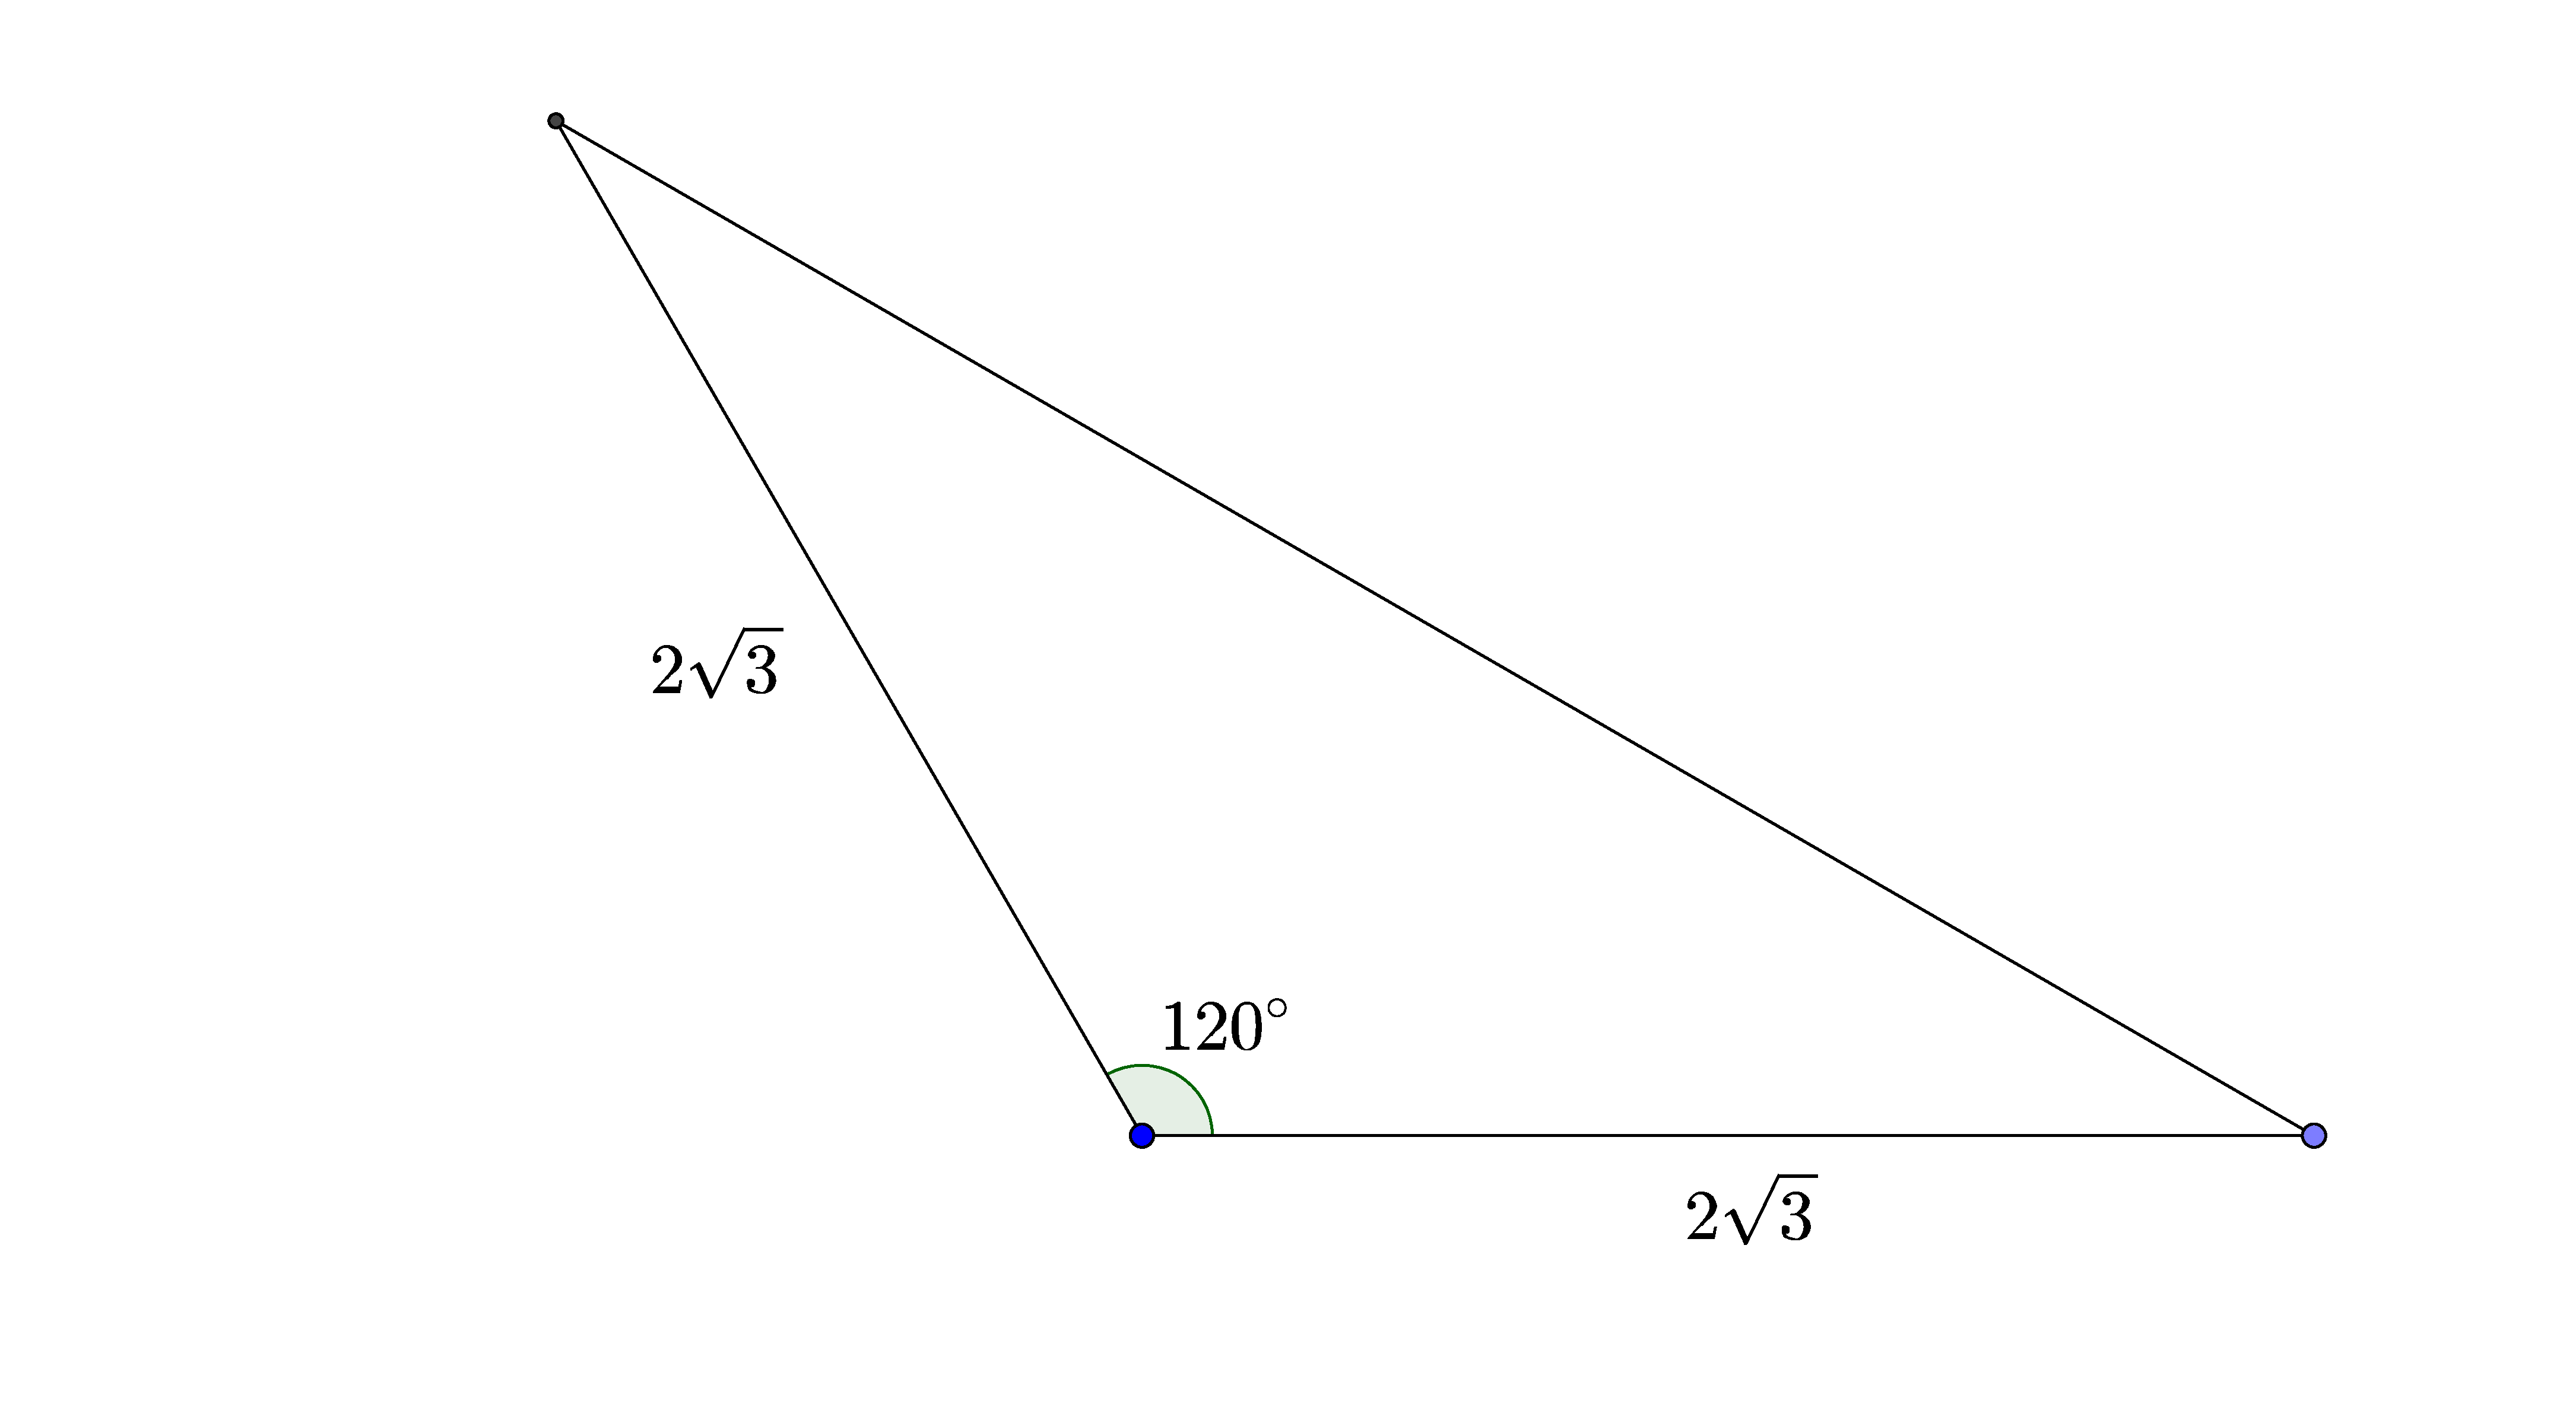
\includegraphics[scale=0.15]{heron.pdf}
\end{center}

\begin{enumerate}

\item Calculate the area of this triangle using the following theorem:\\

{\bf Heron's Formula:} The area of a triangle with sides of length $a$, $b$, and $c$ is $A=\sqrt{s(s-a)(s-b)(s-c)}$ where $s=\frac{a+b+c}{2}$

\ifans\fbox{\parbox{1\linewidth}{Using the Law of Cosines, the missing side of the triangle has length 6.  So, it follows that $a=2\sqrt{3}$, $b=2\sqrt{3}$, $c=6$, and $s=2\sqrt{3}+3$.  Appealing to Heron's Formula gives:
\begin{align*}
A&=\sqrt{s(s-a)(s-b)(s-c)}\\
&=\sqrt{\left(2\sqrt{3}+3\right)\left(2\sqrt{3}+3-2\sqrt{3}\right)\left(2\sqrt{3}+3-2\sqrt{3}\right)\left(2\sqrt{3}+3-6\right)}\\
&=\sqrt{\left(2\sqrt{3}+3\right)(3)(3)\left(2\sqrt{3}-3\right)}\\
&=3\sqrt{\left(2\sqrt{3}+3\right)\left(2\sqrt{3}-3\right)}\\
&=3\sqrt{3}
\end{align*}
}} \fi

\item Calculate the area of this triangle using the formula $A=\frac{1}{2}bh$.

\ifans\fbox{\parbox{1\linewidth}{Dropping a perpendicular from the upper vertex forms a 30-60-90 triangle.  Since the hypotenuse has length $2\sqrt{3}$, we must scale all other sides of the triangle accordingly, as shown in the following figure:
\begin{center}
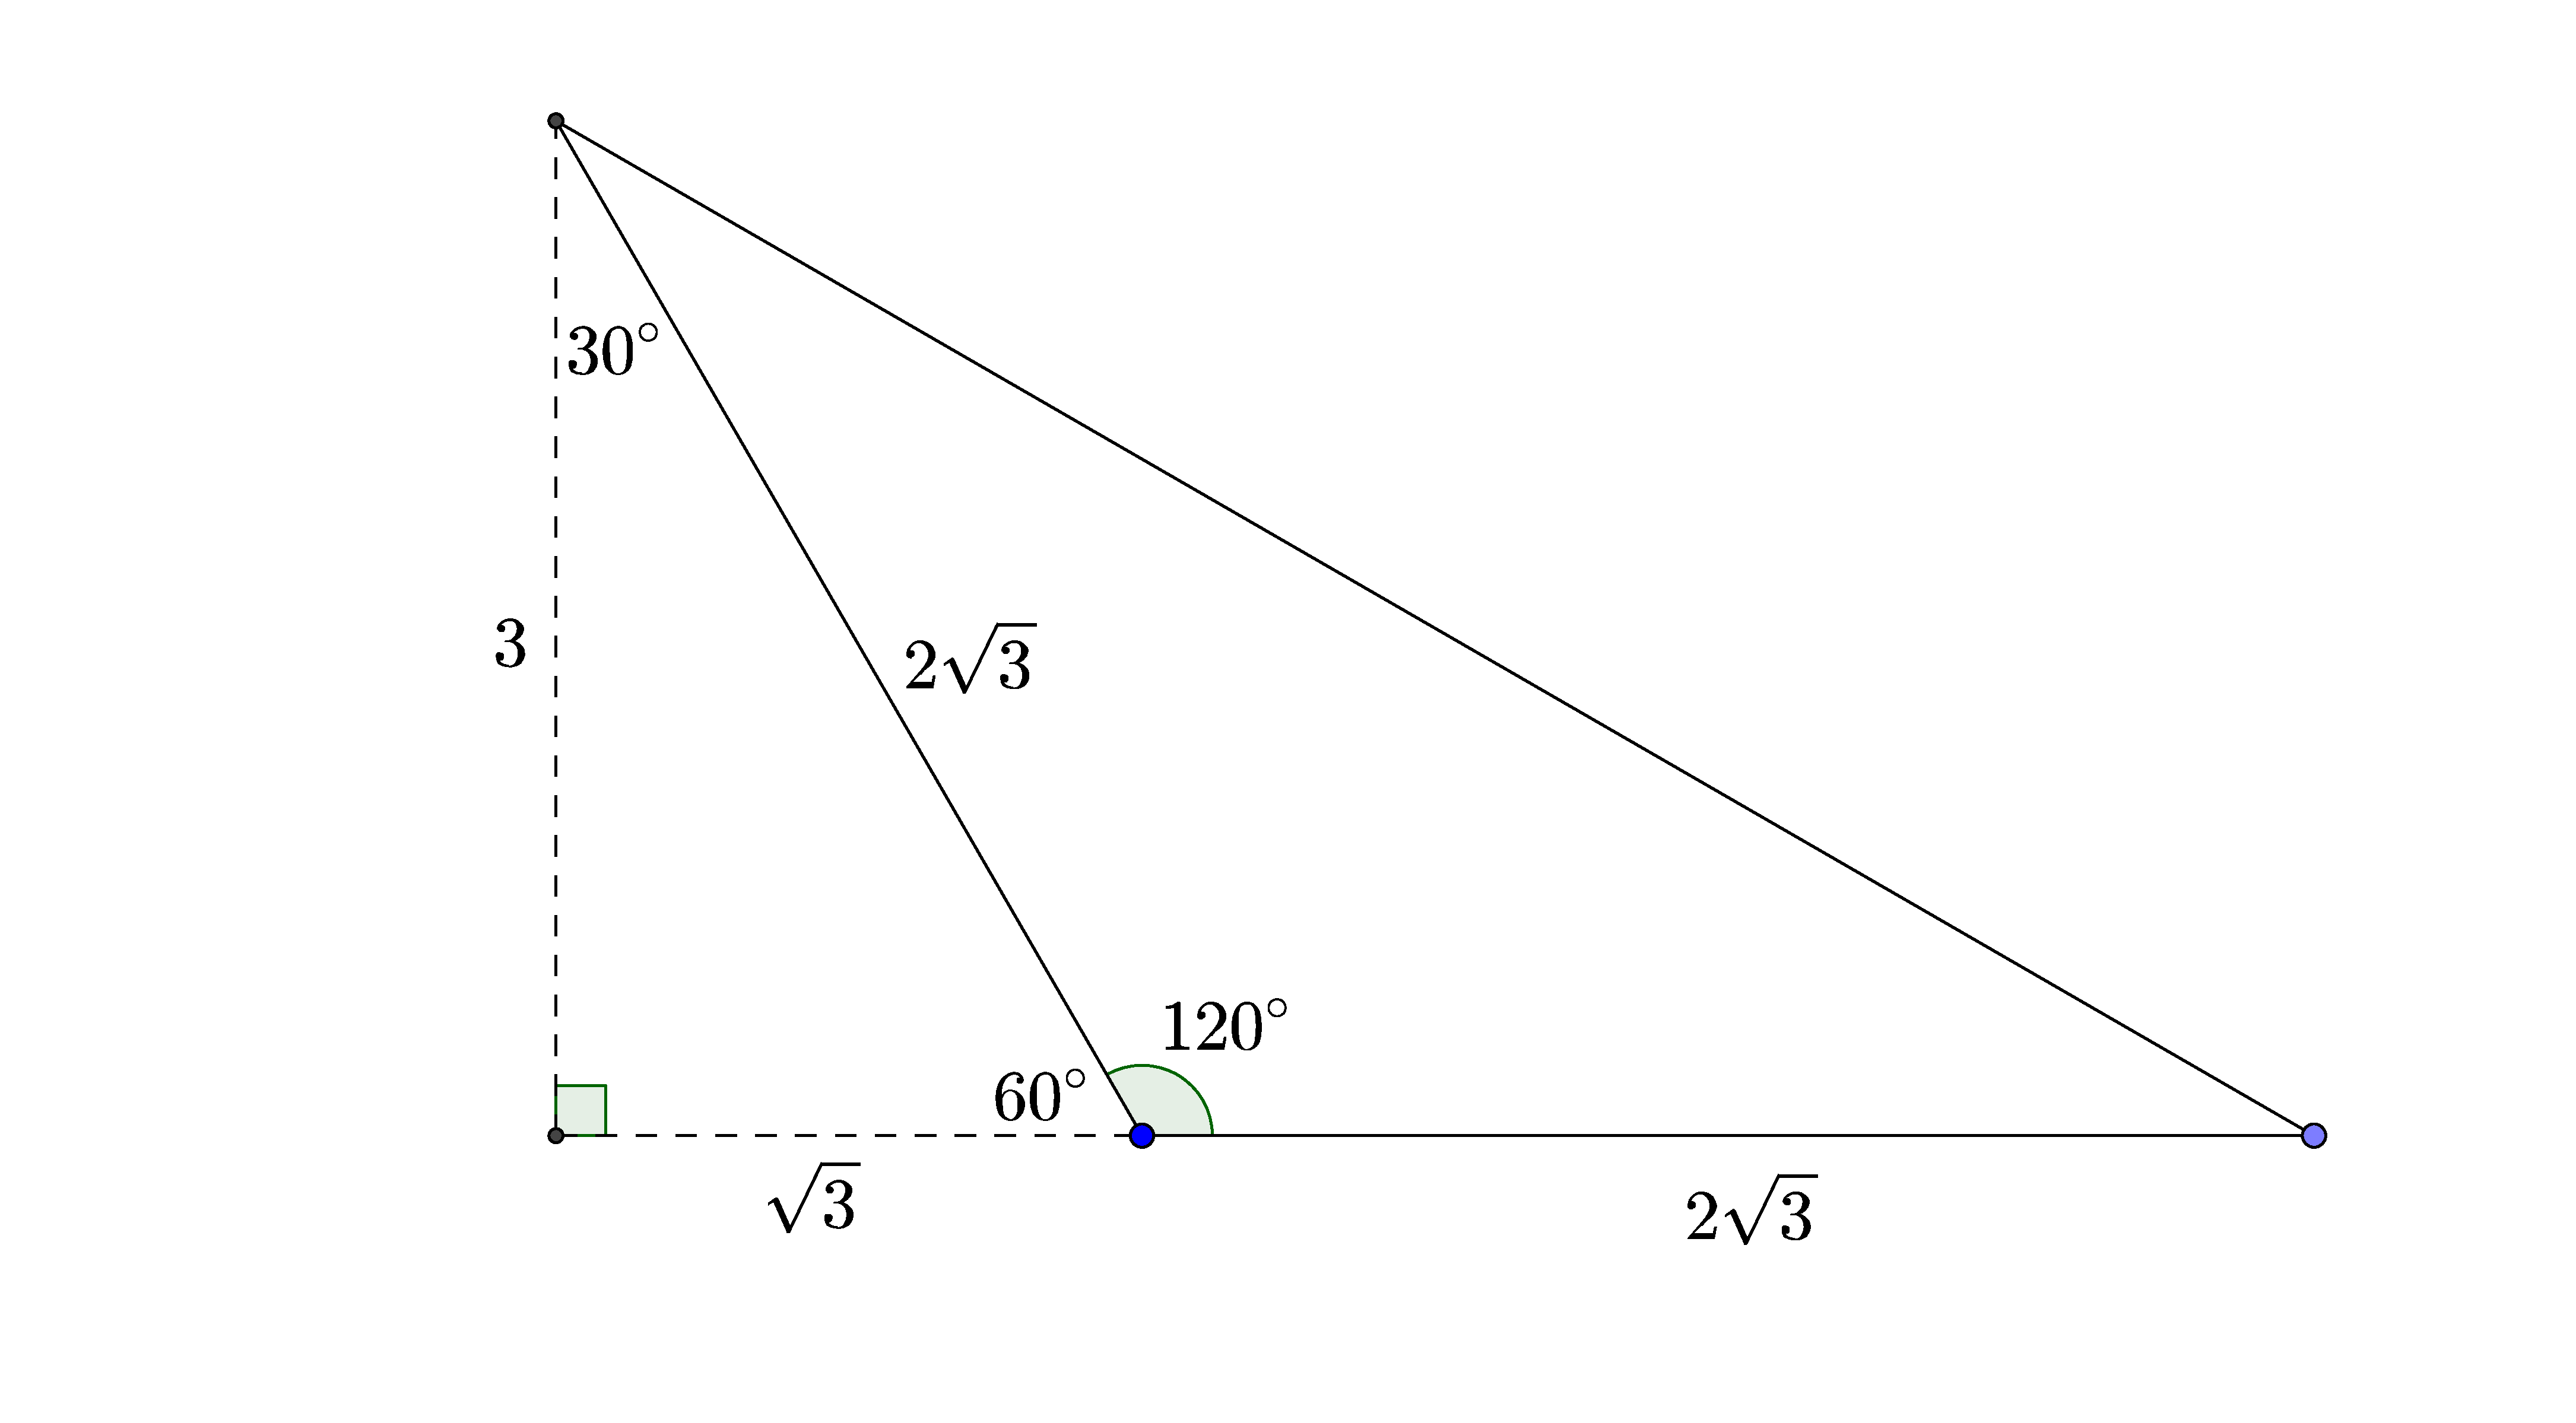
\includegraphics[scale=0.15]{heron1.pdf}
\end{center}
Thus,
\begin{align*}
A&=\frac{1}{2}bh\\
&=\frac{1}{2}\left(2\sqrt{3}\right)(3)\\
&=3\sqrt{3}
\end{align*}
}} \fi

\end{enumerate}

\end{enumerate}

\end{document}